\documentclass[11pt,twocolumn,varwidth=true,a4paper,fleqn]{article}
\usepackage{fullpage}
\usepackage{url}
\usepackage[margin=1.1in]{geometry}
\usepackage{graphicx}
\usepackage{csvsimple}
\usepackage{varwidth}
\usepackage{array}
\usepackage{float}
\usepackage{amsmath}
\usepackage{pgfplotstable}
\usepackage{amsmath }
\usepackage[T1]{fontenc}

\usepackage{authblk}

\author[1]{Bernstein Ran}
\author[2]{Shafir Tal}
\author[3]{Tsachor Rachelle}
\author[4]{Studd Karen}
\author[1]{Schuster Assaf}
\affil[1]{Department of Computer Science, Technion I.I.T, Haifa, Israel}
\affil[2]{The Graduate School of Creative Arts Therapies, University of Haifa}
\affil[3]{School of Theatre \& Music, The University of Illinois at Chicago}
\affil[4]{School of Dance, George Mason University}



\begin{document}
\nocite{*}
\newcolumntype{M}{>{\begin{varwidth}{3cm}}l<{\end{varwidth}}}


\title{Laban Movement Analysis using Kinect Sensor}
\maketitle
\begin{quote}{``Man moves in order to satisfy a need.`` ---\textup{Rudolph Laban}}
\end{quote}
\begin{abstract}
\textbf{Laban Movement Analysis (LMA), developed in the dance community
over the past seventy years, is an effective method for observing, describing, notating, and interpreting human
movement to enhance communication and expression in everyday and professional life.
Many applications that use motion capture data might be significantly
leveraged if LMA was automatically conducted on them.
This paper presents an automated machine learning based method, that recognize
the Laban qualities from motion capture skeletal recordings. The method is
demonstrated on the output of Microsoft's Kinect V2 sensor. The method has
succeed getting over 60\% of recall and precision rate averaged over the
qualities.}
\end{abstract}
\section{Introduction}
\subsection{Motivation for LMA}
LMA is a formal language for motion description 
invented by Rudolf Laban \cite{Laban} in the middle of the 20th 
century. LMA describes, interprets and documents mental 
states from both conscious and unconscious human 
motion based on Laban�s theories of Body, Effort, Shape, 
and Space. LMA has been used in the fields of dancing, 
acting, athletics, physical therapy, and psychology and 
behavioral science. Laban exercises are based on the belief that by observing and analyzing 
movements, both conscious and unconscious, it is possible to recognize the objectives 
of the mover and to become aware of an inner attitude that precedes an action. Laban 
helps actors create momentary moods and long-standing personality characteristic 
through movement. For example, LMA work investigates the Effort properties -
Flow, Space, Time and Weight of all movement and helps actors think specifically about why their character may move in a jerky, fast, light and 
direct manner verses a heavy, slow, indirect and uninterrupted manner: 
\begin{itemize}
\item
Flow: Bound or Free 
\item
Space: Direct or Indirect 
\item
Time: Sudden or Sustained 
\item
Weight: Strong or Light 
\end{itemize}
\begin{figure*}[ht]
\centering
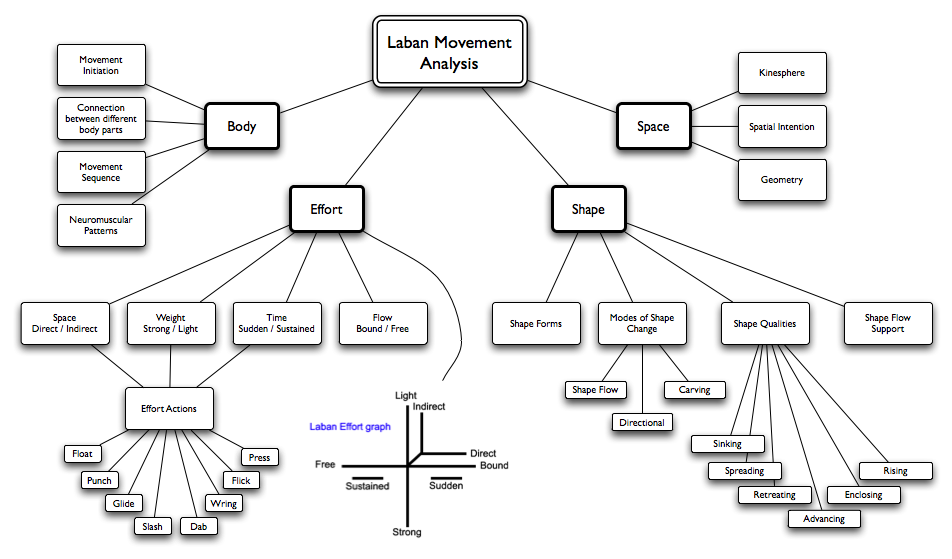
\includegraphics[width=\textwidth]{laban.png}
\caption{Laban movement analysis main axes. Adopted from \cite{LMA}}
\label{labanTree}
The whole hierarchy of LMA is described in figure number \ref{labanTree}.
\end{figure*}
Our main motivation for LMA comes from the correlation between LMA and emotional
movements and emotions as stated by Shafir \cite{shafir}.
From that reason we narrowed our mission on the recognition of  only 18 Laban
qualities (as listed in table \ref{mixedSummary}) that have been found as
predictive for emotions by Shafir.

\subsection{Kinect sensor data}
This following figure shows the skeleton that is provided by the Kinect's
software development kit that were use in this paper.
\begin{figure}[h]
\centering
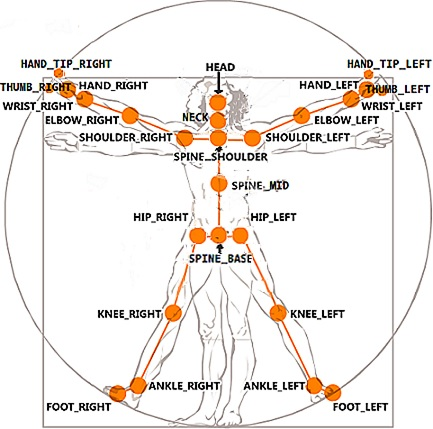
\includegraphics[width=60mm]{skeleton.jpg}
\caption{Skeleton positions relative to the human body}
\label{skeleton}
\end{figure}
Once the skeleton is detected, the 3D coordinates of all joints of user�s body 
� with the exception of joints, that are not visible (e.g. a user�s hand is
behind his back) are provided.
As seen in figure \ref{Coordinate}, the coordinates are in a �real-world�
coordinate system, that has the beginning [0,0,0] in the sensor, x,y and z-axis goes as shown on the picture below and the units are millimeters. 
\begin{figure}[h]
\centering
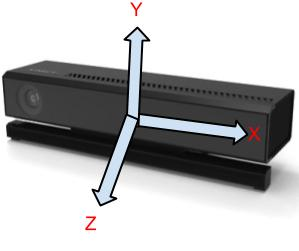
\includegraphics[width=60mm]{KinectV2CoordinateSystem.jpg}
\caption{Kinect Coordinate System}
\label{Coordinate}
\end{figure}

\subsection{Related Work}
Several attempts were made in order to recognize Laban qualities,
most of them were made for emotion recognition in the context of Human Robot Interaction (HRI).
Martin at al. \cite{martin} has analysed the importance of gestures in emotion
recognition for HRI. Masuda et al. generated emotional body motion for a human 
form robot \cite{Masuda}. Rett et al. proposed a human motion recognition 
system using a Bayesian reasoning framework \cite{Rett}. Gabel et al.
\cite{gabel2012full} used the Kinect for gait analysis. Zacharatos et al.
\cite{Zacharatos} and Kim at al. \cite{kim} got
inspiration from LMA for emotion recognition using the Kinect, but their focus was on emotions, not
on LMA.
Common in these studies, computational LMA offers some evidence that motion conveys emotional information, and this information 
allows such systems to estimate qualitative changes of motion.
Kim et al. performed first steps in this direction with the Kinect sensor, in 
this paper we extend such kind of work.

\section{Dataset Creation and Extraction}
\subsection{Clips Collection}
Two main datasets were collected: 
\begin{itemize}
  	\item 
	CMAs dataset - includes 7 CMAs performing in about
	of 80 clips each (550 clips total). Every clip is 3 seconds long, and the CMA
	performs random activity in it. To achieve uniform distribution of the Laban
	qualities over the dataset, in every clip the CMA was asked to perform
	several specific qualities, and nothing but them.
	\item 
	Non CMAs dataset - includes 3 subjects without a background in movement
	analysis, performing 20 clips each. Every clip is 3 seconds long too, where the
	in every clip the subject was asked to perform one out of two operations.
\end{itemize}
\subsection{Clips Labeling}
To achieve a ground truth labeling for the two datasets, every clip was tagged by
a committee of 2-3 CMAs that determined which Laban qualities appear in the
clip. The usage of a committee decision instead of the subjective opinion of one
CMA decreases the labeling noise and considered as ground truth, especially for
the fact that there is no really ground truth in such a non quantitative mission
as the LMA.
\subsection{Feature Extraction}
Due to unequal length of clips, all the features that were extracted are in
whole clip granularity.
\subsubsection{General low level features}
For every joint in the skeleton the angular velocity, acceleration and jerk were
extracted, and for each one of them the mean, variance, skew and kurtosis were
extracted (the extraction of the last four moments is denoted as $\phi$). 
\subsubsection{Shape: Sagittal}
In this quality a separation between Advance and Retreat. The quantification of
this quality was done by projecting the speed vector of the Center Of Mass (COM)
on the vector of the front of the body. The COM was approximated in this case
by the average of all of the joints. The front of the body was approximated by
the perpendicular vector to the the vector between the Left Shoulder (LS) and
the Right Shoulder (RS).
\\If $\vec{P}_{j}(t)$ is the vector of the position of joint j in time t in
a clip with n frames, and $ \alpha_{j}$ is a coefficient proportional to the
mass around of the joint:
\\
\\$\vec{P}_{COM}(t) = \sum_{j \in Joints} \alpha_{j}\vec{P}_{j}(t)
\\
\\\vec{P}_{shoulders}(t)=\vec{P}_{LS}(t)-\vec{P}_{RS}(t)$
\\
\\\[ \vec{P}_{front}=\vec{P}_{shoulders}\left( \begin{array}{ccc}
0 & 0 & 1 \\
0 & 1 & 0 \\
-1 & 0 & 0 \end{array} \right)\]
\\
\\
$S_{sag}(t) = \vec{P}_{COM}(t)\cdot\vec{P}_{front}(t)$
\\
\\
$\vec{F}_{sag} = \phi([S_{sag}(1), \ldots S_{sag}(n)])$
\\\\
Where $\phi$ is the moments extraction.
\subsubsection{Shape: Horizontal}
Here the separation is between spreading and enclosing in the horizontal axis
This quality was quantified by measuring the average distance of the joint from
the the vertical axis of the body that spreads from the Head (H) along the Spine
Base (SB).
This axis was approximated with the Kinect's horizontal axis(y), what made the
distance measured in the projection of the joints on the XZ plane.
\\
\\$d_{j} = \frac{\left|(\vec{P}_{j}-\vec{P}_{SB})\times
(\vec{P}_{j}-\vec{P}_{H})\right|}{\left|\vec{P}_{H}-\vec{P}_{SB}\right|}
\\
\\S_{horiz}(t) = \sum_{j \in Joints} d_{j}(t)
\\
\\\vec{F}_{horiz} = \phi([S_{sag}(1), \ldots S_{sag}(n)])$
\\\\
Where $\phi$ is the moments extraction.
\subsubsection{Shape: Vertical}
Here the separation is between Rise and sink.
This quality was quantified by measuring the average distance on axis y of each
joint from the COM. This quantification comes from the assumption that the body
is ``longer'' when rising.
\\
\\$S_{vert}(t) = \sum_{j \in Joints}
\left|\vec{P}_{j}-\vec{P}_{COM}\right|
\\
\\\vec{F}_{vert} = \phi([S_{sag}(1), \ldots S_{sag}(n)])$
\\\\
Where $\phi$ is the moments extraction.
\subsubsection{Effort: Time}
Here the separation is between Sudden or Sustained. This quality was 
quantified by the skew of the acceleration, relaying on the belief that the
acceleration of a sudden movement will be more left skewed in the the beginning
of the movement (where the acceleration is positive).
\subsubsection{Effort: Space}
Here the separation is between direct and indirect. This quality was 
quantified by the angle between the movement vector of a joint to the next one,
relaying on the belief that in direct movement every vector will be in
the same direction as the last (the angle between them is small).
\\If $\vec{P}_{j}(t)$ is the vector of the position of joint j in time t, the
movement vectors are:
\\\\$\vec{V}_{j}(t) = \vec{P}_{j}(t+1) - \vec{P}_{j}(t)
\\\\The angles between them are calculated with inner products:
\\\\\vec{A}_{j}(t) = \vec{V}_{j}(t+1) \cdot \vec{V}_{j}(t)$


\subsection{Performance Evaluation}
There are 18 labels (Laban qualities) that every recording can get, but
a typical gesture usually includes about 3 qualities, what means that there is
more than 90\% chance that a quality won't characterize the gesture. Due to
this sparsity, a simple accuracy is not a relevant metric for the performance
evaluation because one can get 90\% accuracy by stating that for every recording
non of the qualities appear. A better evaluation have to combine the precision
and recall rates of the classifier. The way that the last two were combined is
with the usage of F one score:
\\
\\$F_{1} = \frac{2\cdot precision\cdot recall}{precision+recall}$
\subsection{Feature Selection}
	Every clip is extracted into a vector of 6120 features. Most of
	them are noisy or redundant. For that reason a massive feature selection is
	needed. The feature selection is done in three stages:
	\begin{itemize}
		\item
		Computing the Anova F-value for every feature over the training set. Cross validation was used to determine the optimal amount of features that should be
		left. As it seen in figure  \ref{selection}, The result was that the filtering
		of the vectors outperformed the usage in non filtered vectors, where using the
		top 4\% of features is optimal.
		\begin{figure}[ht!]
			\centering
			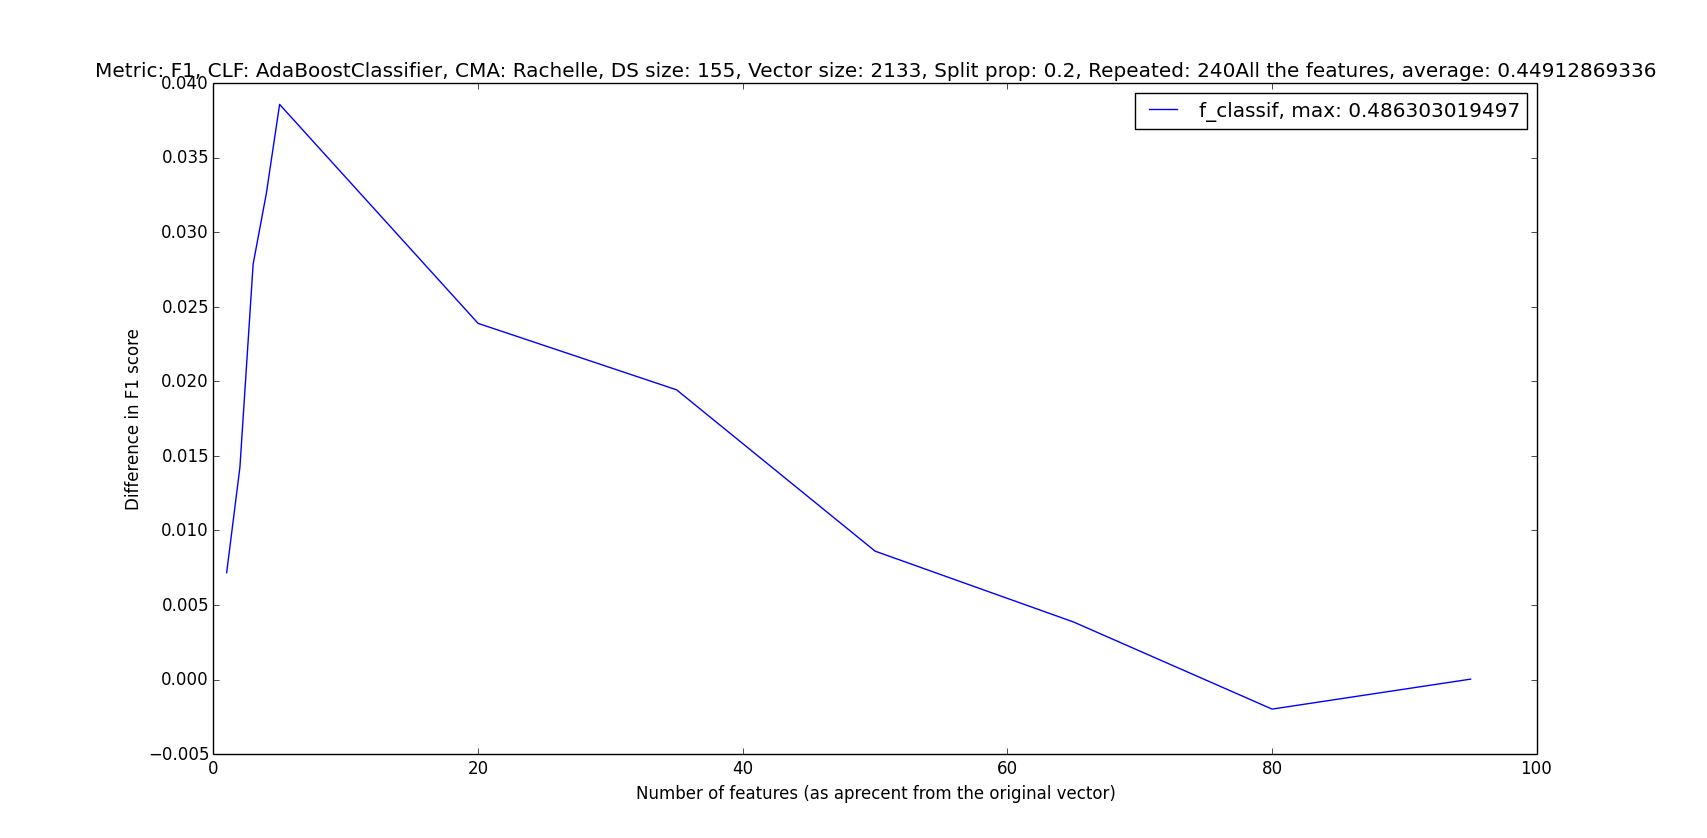
\includegraphics[width=70mm]{featureSelection.png}
			\caption{Influence of the percent of features that were selected based on
			statistical significance on the F1 score.
			The blue line is the difference between the score with and without feature
			selection. It can be seen that the optimal amount to select is 4\%}
			\label{selection}
			\end{figure}
		\item
		\ref{igFromFclassif}
		The second phase of feature selection is conducted by information gain rating
		of the features. As it seen in figure  \ref{igFromFclassif}, the optimal ratio
		was selecting the top 60\% out of the features that have been selected by
		statistical significance.
		 \begin{figure}[h]
			\centering
			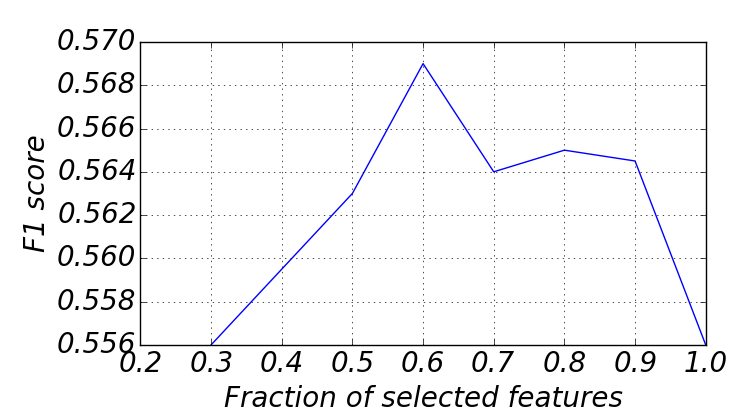
\includegraphics[width=70mm]{igFromFclassif.png}
			\caption{Influence of the proportion of Information based selection from the
			subset of features that was chosen by the ANOVA selection. The optimal ratio
			was 60\%.}
			\label{igFromFclassif}
		\end{figure}
		\item
		The third phase of feature section was made by Least Absolute Shrinkage and
		Selection Operator (LASSO).
	\end{itemize}
	Example for qualities and their most significant Features is shown in 
	table number \ref{bestFeatures}. The ``Information Gain'' metric that is used
	in the table, is defined:
	\begin{equation*}
	       IG(T,f) = H(T) - H(T|f)
	\end{equation*} 
	Where T is the training set, f is a feature and H() is the information
	entropy of a dataset.
	 \begin{table*}[ht]
	   \centering
	   \csvautotabular{rankFeatures.csv}
	   \caption{Example for several qualities and the feature that has been found
	   the most informative for them. ``Relative position'' stands for the
	   position of the joint relatively to ancestor joint in the joints hierarchy.}
	   \label{bestFeatures}
	\end{table*}

\section{Experimental Setups and Results}
\subsection{Multilabel classification}
Multilabel learning deals with the problem where each instance is associated
with multiple labels simultaneously, where the number of labels is not fixed
between instance to instance. The task of this learning paradigm is to predict
the label (Laban quality) set for each unseen instance (skeletal recording), 
through analyzing training instances with known label sets. The multilabel
approach that was taken in this paper is to break the whole LMA problem into 18
binary classification tasks - one for every Laban quality - where every binary
decision is if the quality exists or not.
\\The next following subsections will be describe several experimental setups
where the results in every one will stand as a base line for the next setup.
\subsection{Per CMA evaluation}
	In this experiment both of the train and test datasets are taken from the same
	CMA. The average performance over the different CMAs are shown in table
	\ref{oneCMASummary}. The performance on every Laban quality separately
	is demonstrated on a dataset of one of the CMAs in figure \ref{oneCMAFinal}.
	\begin{table}[H]
	  	\centering
		\begin{tabular}{|p{1.6cm}|p{0.9cm}|p{0.9cm}|p{0.9cm}|p{0.9cm}|}
		\hline
		Algorithm /Metric&Preci-sion&Recall&F1&F1 SD\\\hline
		Chance&0.15&0.50&0.23&0.01\\\hline
		Nearest Neighbors&0.30&0.24&0.26&0.05\\\hline
		LinearSVC &0.35&0.39&0.37&0.04\\\hline
		Label Balancing&0.39&0.42&0.41&0.05\\\hline
		LogLoss&0.40&0.43&0.43&0.04\\\hline
		Lasso&0.41&0.48&0.44&0.05\\\hline
		Statistic Feature Selection&0.44&0.51&0.48&0.09\\\hline
		IG Feature Selection&0.48&0.59&0.53&0.09\\\hline
		\end{tabular}
		\caption{Recall, precision and F1 score of each step in the algorithm
		development. Every CMA was evaluated separably. The
		results are the average performance and standard deviation (SD) over the CMAs.}
	   \label{oneCMASummary}
	\end{table}

	\begin{figure*}[ht!]
		\centering
		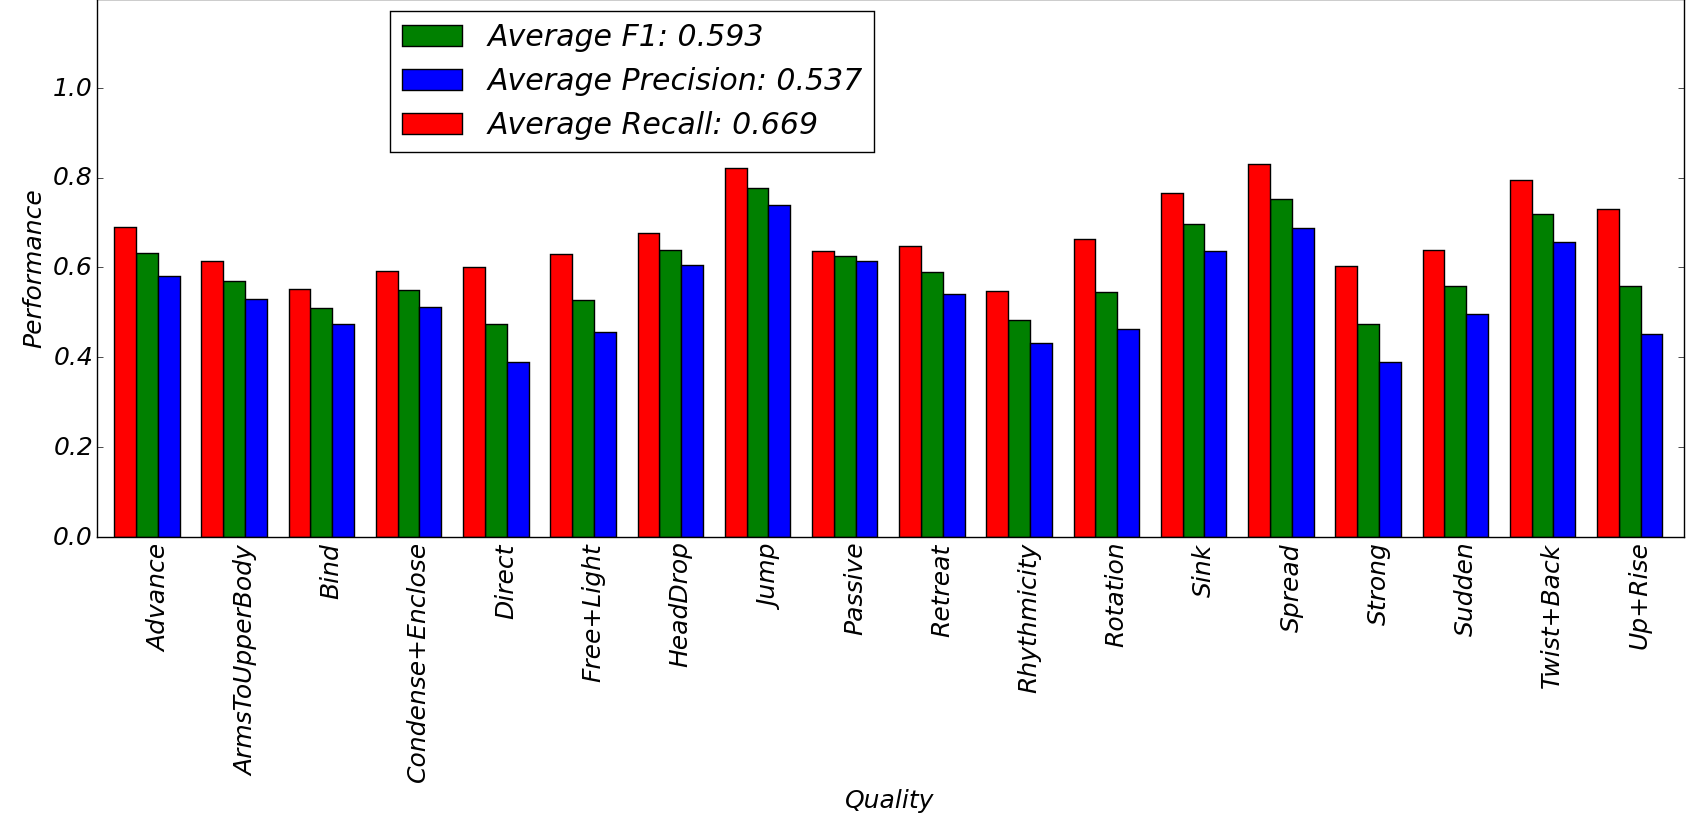
\includegraphics[width=\textwidth, height=60mm]{oneCMAFinalWithoutTitle.png}
		\caption{Recall, precision and F1 score of each Laban quality separately. The
		evaluation was made on a dataset that was captured on only one CMA.}
		\label{oneCMAFinal}
	\end{figure*}
	
\subsection{Mixed datasets evaluation}
	In this experiment the datasets of all of the CMAs were mixed. In the learning
	and testing process the origin (CMA) of the sample was ignored. 
\subsubsection{Single task learning as a baseline}
	\begin{table}[ht!]
	  	\centering
		\begin{tabular}{|p{1.6cm}|p{0.9cm}|p{0.9cm}|p{0.9cm}|p{0.9cm}|}
		\hline
		Algorithm /Metric&Preci-sion&Recall&F1\\\hline
		Chance&0.15&0.50&0.23\\\hline
		Nearest Neighbors&0.41&0.235&0.3\\\hline
		LinearSVC &0.4&0.43&0.418\\\hline
		Label Balancing&0.394&0.47&0.43\\\hline
		LogLoss&0.4&0.46&0.43\\\hline
		Lasso&0.4&0.45&0.42\\\hline
		Statistic Feature Selection&0.462&0.69&0.55\\\hline
		IG Feature Selection&0.46&0.71&0.56\\\hline
		\end{tabular}
		\caption{Recall, precision and F1 score of each step in the algorithm
	   development}
	   \label{mixedCMASummary}
	\end{table}
		
\subsubsection{Multi task vs Single task learning}
We found that multitask learning for all the 18 qualities together overcome in
its performance learning a classifier to each problem separately. For the
multitask mission we used Multitask Elastic Net (MEN) regularization, which is
the multitask from of Zou at al. \cite{Zou} regularization, where the
optimization objective for the MEN is:
\\
\begin{equation*}
	\|Y - XW\|^2_F+\lambda_1\cdot\|W\|_{2,1}+\lambda_1\cdot\|W\|^2_F
\end{equation*}       
\\
$\lambda_1$ is generalization hyper parameter, and $\lambda_2$ is hyper
parameter that balance between the $L_{2,1}$ and the rest.
Where:
\\
\begin{equation*}
        \|W\|_{2,1} = \sum_i \sqrt{\sum_j w_{ij}^2}
\end{equation*} 
    i.e. the sum of norm of each row (also known as mixed norm), and 
\begin{equation*}
        \|W\|^2_F = \sum_i{\sum_j w_{ij}^2}
\end{equation*}     
	i.e. the Frobenius norm. 

Feature selection was made by averaging the statistical significance of each
feature with a respect to different task (Not like in the single task learning
flow, there every task had its own feature selection). As it seen in table
\ref{MultitaskVsSeparated} the multitask setting improved the F score in 7\%,
fact that indicates that the tasks are correlated and that more might be learned
from the small dataset when using this setting.	
 	\begin{table}[H]
	  	\centering
		\begin{tabular}{|p{1.8cm}|p{1.8cm}|p{1.8cm}|}
		\hline
		Metric&Single task&Multitask\\\hline
		Precision&0.46&\textbf{0.59}\\\hline
		Recall&\textbf{0.71}&0.65\\\hline
		F1&0.56&\textbf{0.6}\\\hline
		\end{tabular}
		\caption{Multitask vs Single task learning performance evaluation on mixture
		of CMAs dataset.}
	   \label{MultitaskVsSeparated}
	\end{table}

\subsubsection{Performance of every quality in multitask setting}
The In table \ref{mixedSummary} are shown the performance of every quality in
multitask setting. 
\begin{table}[ht!]
	  	\centering
		\begin{tabular}{|p{3cm}|p{0.9cm}|p{0.9cm}|p{0.9cm}|}
		\hline
		Quality&Precis-ion&Recall&F1 score\\\hline
		Jump&0.89&0.81&0.85\\\hline
		Twist+Back&0.69&0.85&0.76\\\hline
		Sink&0.62&0.79&0.69\\\hline
		Rhythmicity&0.59&0.72&0.65\\\hline
		Spread&0.55&0.76&0.64\\\hline
		Head drop&0.60&0.66&0.63\\\hline
		Rotation&0.66&0.60&0.63\\\hline
		Free and Light&0.45&0.94&0.61\\\hline
		Up and Rise&0.67&0.54&0.60\\\hline
		Condense and Enclose&0.44&0.84&0.58\\\hline
		Arms To Upper Body&0.67&0.54&0.60\\\hline
		Advance&1.00&0.38&0.55\\\hline
		Retreat&0.50&0.59&0.54\\\hline
		Passive&0.40&0.85&0.54\\\hline
		Bind&0.44&0.61&0.51\\\hline
		Direct&0.56&0.49&0.52\\\hline
		Sudden&0.61&0.41&0.49\\\hline
		Strong&0.29&0.42&0.34\\\hline
		\textbf{Average}&\textbf{0.59}&\textbf{0.65}&\textbf{0.60}\\\hline
		\textbf{SD}&\textbf{0.17}&\textbf{0.17}&\textbf{0.11}\\\hline
		\end{tabular}
		\caption{Recall, precision and F1 score of each Laban quality on a CMA
		   mixture dataset. The learning was done in a multitask setting. The number of
		   features that didn't become zero after the mixed norm regularization is
		   282 (same features for all of the tasks). The F1 average and standard
		   deviation over the qualities is shown in the last row of the table.}
	   \label{mixedSummary}
	\end{table}
The mixed norm term in the MEN optimization problem promotes
sparsity in the weights matrix $W$ in the way that every row is or all zeros or
all non-zeros. This affect is a kind of collective (over the tasks) feature
selection. The collective decision which features to select, enhanced the
generalization ability of the model, especially in the qualities that
performed worse in the single task learning (e.g. strong and sudden).

\subsection{Evaluation on a new CMA}
In this experiment the test set was taken from a CMA that didn't appear in
the train set. As it shown in table
\ref{domainAdaptationBaseLine}, there is a degradation in the performance on the new CMA.
 \begin{table}[H]
  	\centering
	\begin{tabular}{|p{1.8cm}|p{1.8cm}|p{1.8cm}|}
	\hline
	Metric&Average Score&Standard deviation\\\hline
	Precision&0.41&0.053\\\hline
	Recall&0.53&0.089\\\hline
	F1&0.457&0.064\\\hline
	\end{tabular}
	\caption{Qualities detection performance on a new subject. In every
	trial one CMA was the test set, while the classifier was learned from the
rest of the CMAs.}
   \label{domainAdaptationBaseLine}
\end{table}
We blame the degradation on the great variability that we got between clips from
one CMA to others. Every CMA performed different gestures, in different postures
(some sitting while some standing) and in different context (some were dancing
while some where acting).
This great variability motivated us to work in Domain Adaptation (DA) setting.

\subsection{Validation on ordinary people}
The final validation was made ordinary people (non CMAs). We
designed several daily actions (greeting friends, playing with a balloon etc.),
and the CMAs committee has tagged the clips. This dataset was small and
concentrated on the elements that are shown in table number \ref{nonCMAs}.

\begin{table}[H]
\centering
\begin{tabular}{|p{3cm}|p{0.9cm}|p{0.9cm}|p{0.9cm}|}
	\hline
	Quality&Precis-ion&Recall&F1 score\\\hline
	Jump&0.69&0.75&0.72\\\hline
	Spread&0.53&0.82&0.65\\\hline
	Arms To Upper Body&0.5&0.5&0.5\\\hline
	Free and Light&0.53&0.48&0.5\\\hline
	Sink&0.45&0.58&0.5\\\hline
	Condense and Enclose&0.4&0.5&0.45\\\hline
	Rotation&0.3&0.86&0.45\\\hline
	\end{tabular}
	\caption{Performance on ordinary people (non CMAs), that  have been told to
	   perform several tasks.}
\label{nonCMAs}
\end{table}

\section{Conclusion}
Our method has succeed getting over 60\% of recall and precision rate averaged over the
qualities. There are few Laban qualities, such as strong, that we have found that is
more difficult to quantify in bio-mechanical measurements. Over all we believe
that we have succeeded capturing the essence of most of the qualities with a
100\$ sensor, what will make the LMA reachable in places that it have never seen
before.
\bibliographystyle{unsrt}
\bibliography{bib}

\end{document}
